\documentclass[tikz]{standalone}
\usepackage[utf8]{inputenc}

\definecolor{mycolor}{RGB}{12,18,33}

\begin{document}
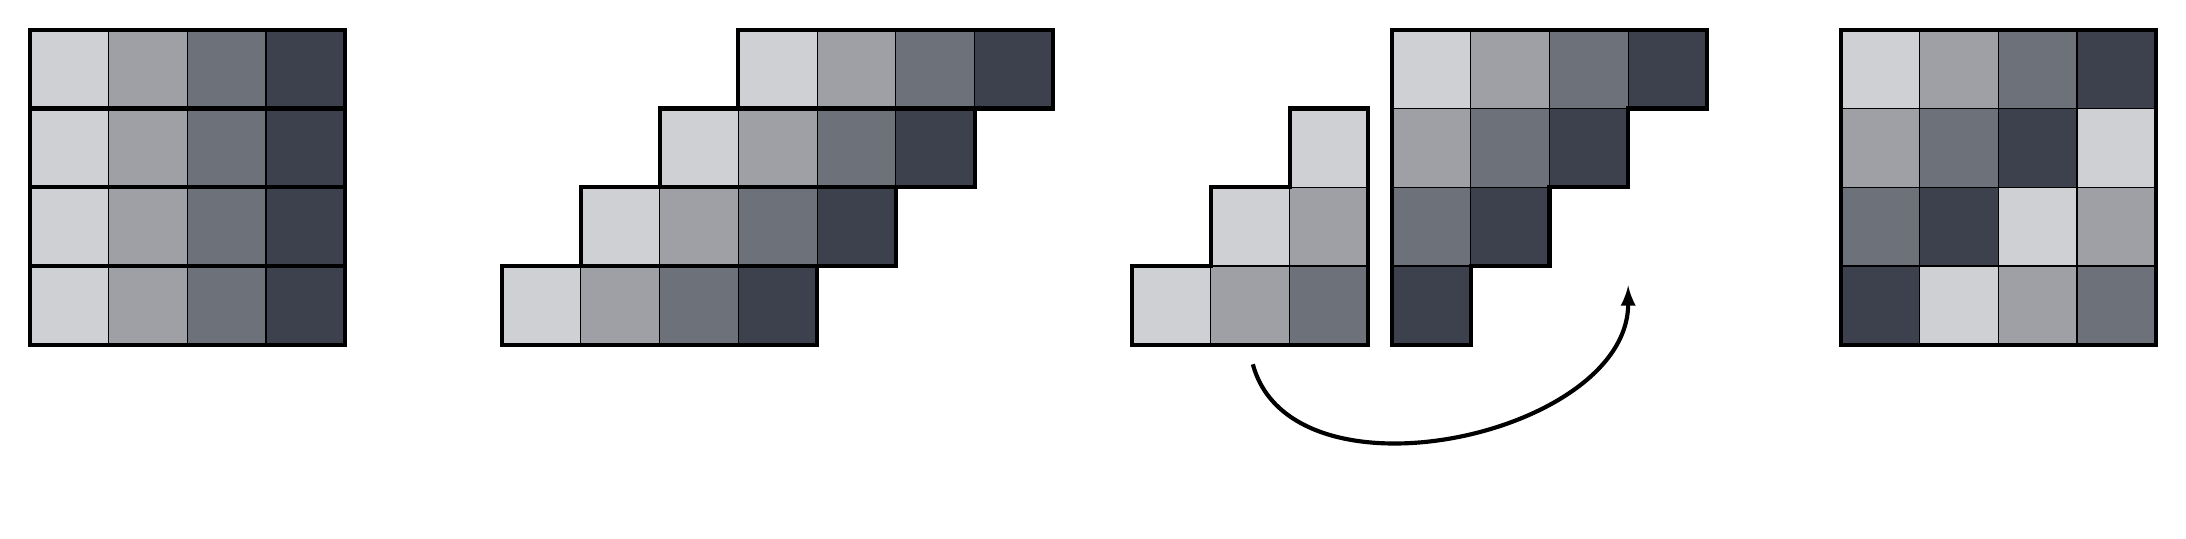
\begin{tikzpicture}
% before SR
\fill[mycolor!20] (0,0) rectangle (1,4);
\fill[mycolor!40] (1,0) rectangle (2,4);
\fill[mycolor!60] (2,0) rectangle (3,4);
\fill[mycolor!80] (3,0) rectangle (4,4);

\draw (0, 0) -- (0, 4);
\draw (1, 0) -- (1, 4);
\draw (2, 0) -- (2, 4);
\draw (3, 0) -- (3, 4);
\draw (4, 0) -- (4, 4);

\draw[line width=1.5pt] (0, 0) rectangle (4, 1);
\draw[line width=1.5pt] (0, 1) rectangle (4, 2);
\draw[line width=1.5pt] (0, 2) rectangle (4, 3);
\draw[line width=1.5pt] (0, 3) rectangle (4, 4);

% shift
\begin{scope}[shift={(9,0)}]

\draw[fill=mycolor!20] (-3,0) rectangle (-2,1);
\draw[fill=mycolor!20] (-2,1) rectangle (-1,2);
\draw[fill=mycolor!20] (-1,2) rectangle (0,3);
\draw[fill=mycolor!20] (0,3) rectangle (1,4);

\draw[fill=mycolor!40] (-2,0) rectangle (-1,1);
\draw[fill=mycolor!40] (-1,1) rectangle (0,2);
\draw[fill=mycolor!40] (0,2) rectangle (1,3);
\draw[fill=mycolor!40] (1,3) rectangle (2,4);

\draw[fill=mycolor!60] (-1,0) rectangle (0,1);
\draw[fill=mycolor!60] (0,1) rectangle (1,2);
\draw[fill=mycolor!60] (1,2) rectangle (2,3);
\draw[fill=mycolor!60] (2,3) rectangle (3,4);

\draw[fill=mycolor!80] (0,0) rectangle (1,1);
\draw[fill=mycolor!80] (1,1) rectangle (2,2);
\draw[fill=mycolor!80] (2,2) rectangle (3,3);
\draw[fill=mycolor!80] (3,3) rectangle (4,4);

\draw[line width=1.5pt] (-3, 0) rectangle (1, 1);
\draw[line width=1.5pt] (-2, 1) rectangle (2, 2);
\draw[line width=1.5pt] (-1, 2) rectangle (3, 3);
\draw[line width=1.5pt] (0, 3) rectangle (4, 4);
\end{scope}

% Tetris: left block
\begin{scope}[shift={(17,0)}]

\draw[fill=mycolor!20] (-3,0) rectangle (-2,1);
\draw[fill=mycolor!20] (-2,1) rectangle (-1,2);
\draw[fill=mycolor!20] (-1,2) rectangle (0,3);
\draw[fill=mycolor!40] (-2,0) rectangle (-1,1);
\draw[fill=mycolor!40] (-1,1) rectangle (0,2);
\draw[fill=mycolor!60] (-1,0) rectangle (0,1);

\draw[line width=1.5pt] (-3,0) --++ (3,0) --++ (0,3) --++ (-1,0) --++ (0,-1) --++ (-1,0) --++ (0,-1) --++ (-1,0) -- cycle;

\node[below] (a) at (-1.5, 0) {};
\end{scope}


% Tetris: right block
\begin{scope}[shift={(17.3,0)}]

\draw[fill=mycolor!20] (0,3) rectangle (1,4);
\draw[fill=mycolor!40] (0,2) rectangle (1,3);
\draw[fill=mycolor!40] (1,3) rectangle (2,4);
\draw[fill=mycolor!60] (0,1) rectangle (1,2);
\draw[fill=mycolor!60] (1,2) rectangle (2,3);
\draw[fill=mycolor!60] (2,3) rectangle (3,4);
\draw[fill=mycolor!80] (0,0) rectangle (1,1);
\draw[fill=mycolor!80] (1,1) rectangle (2,2);
\draw[fill=mycolor!80] (2,2) rectangle (3,3);
\draw[fill=mycolor!80] (3,3) rectangle (4,4);

\draw[line width=1.5pt] (0,0) --++ (1,0) --++ (0,1) --++ (1,0) --++ (0,1) --++ (1,0) --++ (0,1) --++ (1,0) --++ (0,1) --++ (-4, 0) -- cycle;

\node[below] (b) at (3, 1) {};

\end{scope}

\draw[-latex, line width=1.5pt] (a) to[out=-75, in=-90] (b);


% after
\begin{scope}[shift={(23,0)}]

\draw[fill=mycolor!20] (0,3) rectangle (1,4);
\draw[fill=mycolor!20] (1,0) rectangle (2,1);
\draw[fill=mycolor!20] (2,1) rectangle (3,2);
\draw[fill=mycolor!20] (3,2) rectangle (4,3);

\draw[fill=mycolor!40] (0,2) rectangle (1,3);
\draw[fill=mycolor!40] (1,3) rectangle (2,4);
\draw[fill=mycolor!40] (2,0) rectangle (3,1);
\draw[fill=mycolor!40] (3,1) rectangle (4,2);

\draw[fill=mycolor!60] (0,1) rectangle (1,2);
\draw[fill=mycolor!60] (1,2) rectangle (2,3);
\draw[fill=mycolor!60] (2,3) rectangle (3,4);
\draw[fill=mycolor!60] (3,0) rectangle (4,1);

\draw[fill=mycolor!80] (0,0) rectangle (1,1);
\draw[fill=mycolor!80] (1,1) rectangle (2,2);
\draw[fill=mycolor!80] (2,2) rectangle (3,3);
\draw[fill=mycolor!80] (3,3) rectangle (4,4);

\draw[line width=1.5pt] (0,0) rectangle (4,4);

\end{scope}
\end{tikzpicture}
\end{document}